\documentclass[twoside]{article}
\usepackage[utf8]{inputenc}
\usepackage[a4paper, total={6in, 8in}]{geometry}
\usepackage{fancyhdr}
\usepackage[english]{babel}
\usepackage{longtable}
\usepackage{graphicx}
\usepackage{parskip}
\usepackage{multicol}
\usepackage{cite}
\usepackage{pdfpages}

\renewcommand{\familydefault}{\sfdefault}
\newcommand{\gw}{7cm}

\pagestyle{fancy}
\fancyhf{}
\rhead{Hannes Torstensson, Chemistry 2, NA21}
\lhead{The effect of surface area on rate of reaction}
\fancyfoot[RO, LE] {\thepage}

\title{The effect of surface area on rate of reaction}
\author{Hannes Torstensson \\ Chemistry 2, NA21}
\date{PDF generated \today \\ Experiment performed October 20, 2022 \\ Experiment performed with Nicole Hallberg}

\begin{document}
	\maketitle
	\section*{Purpose of the lab}
		Investigating the difference in rate of reaction of vitamin c tablets in tap water as surface area increases. This experiment was done to investigate the veracity of claims made in Steve Owen's "Chemistry for the IB Diploma".
	\section*{Background}
		The reaction is:
		\[C_6H_8O_7 (s) + 3NaHCO_3 (s) \to 3CO_2 + 3H_2O + 3NaC_6H_8O_7\]
		According to collision theory, two particles with sufficient energy and correct orientation must collide to react. This quantity of energy is known as the activation energy, $E_a$. If the particles do not have enough energy they will simply bounce off each other, not reacting. (Owen, 2013)

		Thus, in order for a reaction to take place, two particles with energies equal to or greater than $E_a$ must collide. (Owen, 2013)

		The rate of reaction is affected by collision theory (Owen, 2013). It's factors are:
		\begin{enumerate}
			\item{Concentration of reactants, as concentration of reactants goes up, the likelyhood of two particles colliding also goes up, causing an increase in the rate of reaction. (Owen, 2013)}
			\item{Pressure (only gases), as pressure goes up, the likelyhood of two particles colliding also goes up, as an increase in pressure means that there are more particles per unit of volume, meaning that there will be more collisions, and therefore more reactions. (Owen, 2013)}
			\item{Surface area, as reactions generally only occur at the surface of solids an increase in surface area increses the probability of collision, and therefore also the probability of reaction. (Owen, 2013)}
			\item{Temperature, as temperature goes up, particles have both more energy and more movement, making both collisions and successful collisions (i.e. reactions) more likely. This can be seen by comparing the Maxwell-Botlzman distributions of energies of particles in samples at different temperatures. (Owen, 2013)}
			\item{Catalysis, a catalyst lowers the activating energy, meaning that more collisions result in reactions. (Owen, 2013)}
		\end{enumerate}
		Surface area is the factor that will be investigated in this lab. As the surface area is increased, the amount of reactant available to react at any one time is increased, increasing the "effective concentration" of the reactants, meaning that there is an increased rate of collisions between the reactants, causing an increased rate of reaction. (Owen, 2013)

\section*{Hypothesis}
		As the surface area increases, it is predicted that the rate of reaction will increase.

\section*{Safety}
		No dangerous materials used. No precautions needed.

\section*{Materials}
		The materials used: Scales, 1 50 ml beaker, 1 larger beaker filled with RT water (at least 200 ml), 6 citric acid tablets, 1 timer (cellphone), 1 weighing boat, 1 mortar and pestle, and 1 stick.

\section*{Method}
	\subsection*{Controls}
			Begin by measuring and recording the weight of the tablet using the measuring boat and the scales. Then weigh out 30g of water. Record weight. Start the timer as the tablet is dropped into the water, and record the weight of the contents of the beaker every 10 seconds until you have recorded the same result 4 times consecutively. Repeat three times.

	\subsection*{Experiments}
			Begin by grinding the tablet to a powder using the mortar and pestle. Then scrape the powder into the measuring boat using the stick and record the weight. Then weigh out 30g of water. Record weight. Start the timer as the powder is dropped into the water, use stick to get all the powder into the water, and record the weight of the contents of the beaker every 10 seconds until you have recorded the same result 4 times consecutively. Do not stir. Repeat three times.
	\newpage
\section*{Results}
		Figs. 1 \& 4 are raw representations of the data, figs. 2 \& 5 represent the mass of $CO_2$ released, which is the same as the mass lost from the beaker, or the inverse of figs. 1 \& 4. Figs. 3 \& 6 have their y values calculated with the formula $y = n \times c_{v} $, where $c_{v}$ is the volume of one gram of $CO_2$ at 100kPa and $20^\circ$C\footnote{This was found using the formula $PV=\eta RT$, using $\frac{1}{44.0095}$ as $\eta$, as 44.0095 is the molar mass of $CO_2$ (NIST, n.d.)}, and $n$ is the mass of $CO_2$ generated i grams, which is the same as the loss in mass in the beaker.

	\begin{multicols}{2}
		\begin{center}
			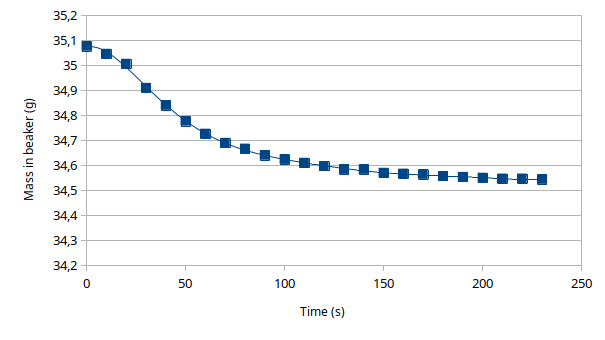
\includegraphics[width=\gw]{ctrl mass_b-time.png}
			\emph{fig. 1} Mean mass remaining in beaker vs time in controls
		\end{center}
		\begin{center}
			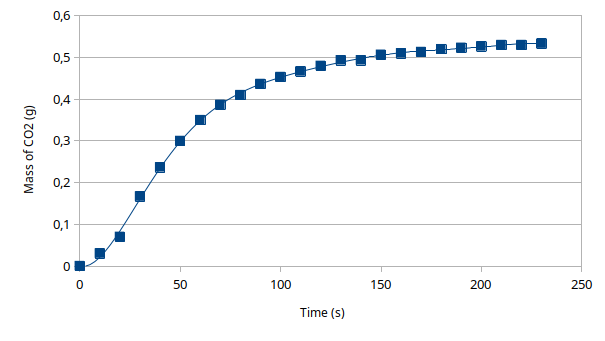
\includegraphics[width=\gw]{ctrl mass_co2-time.png}
			\emph{fig. 2} Mean mass of $CO_2$ generated vs time in controls
		\end{center}
		\begin{center}
			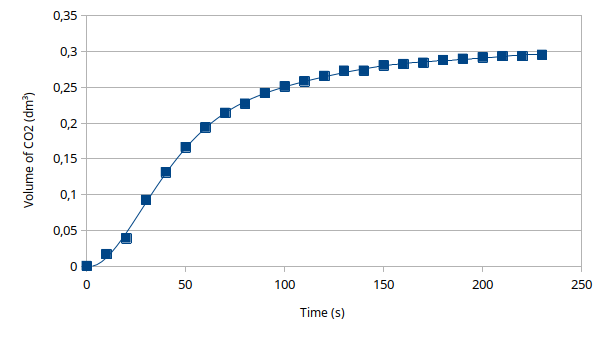
\includegraphics[width=\gw]{ctrl vol-time.png}
			\emph{fig. 3} Mean volume of $CO_2$ generated vs time in controls
		\end{center}
		\begin{center}
			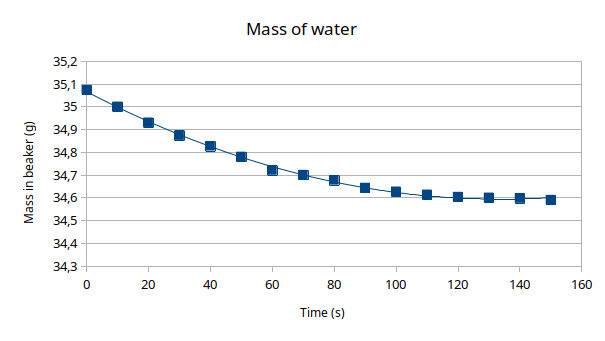
\includegraphics[width=\gw]{exp mass_b-time.png}
			\emph{fig. 4} Mean mass remaining in beaker vs time in experiments
		\end{center}
		\begin{center}
			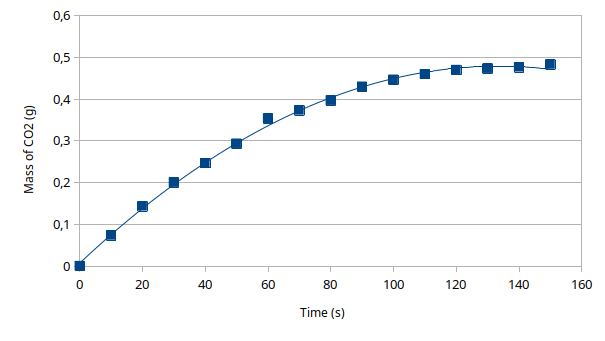
\includegraphics[width=\gw]{exp mass_co2-time.png}
			\emph{fig. 5} Mean mass of $CO_2$ generated vs time in experiments
		\end{center}
		\begin{center}
			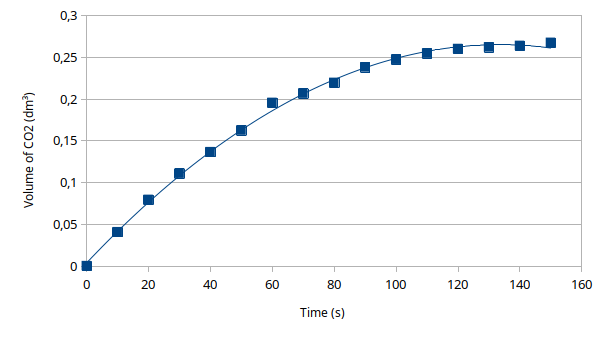
\includegraphics[width=\gw]{exp vol-time.png}
			\emph{fig. 6} Mean volume of $CO_2$ generated vs time in experiments
		\end{center}
	\end{multicols}
	\newpage
\section*{Discussion}
	The hypothesis was confirmed.

	Reaction rates were faster for the experimental runs than for the control runs, as expected. The average overall reaction rate was $3.22 \times 10^{-3}$ grams of $CO_2$ per second for the experimental runs and $2.32 \times 10^{-3}$ grams of $CO_2$ per second for the control runs.\footnote{Found by calculating the secant between $x=0$ and the final unique value.} This is a difference of 38\%.
	
	An interesting note is the shape of the graphs, the best fit lines of the experimental graphs are quadratics that match the data, while the best fit line of the controls begins following the data only when it is a 7th degree polynomial\footnote{A 7th degree polynomial has the form $ax^{7}+bx^{6}+cx^{5}+dx^{4}+ex^{3}+fx^{2}+gx+h=0$}. This is most likely due to the physics of the rate at which the water enters the tablet, and could be an interesting area of further study.

	Sources of uncertainty could be unintentional changes in the other factors in rate of reaction, in this case changes in temperature and concentration. Inaccuracies could also arise from the method, such as the potential effect on the recorded weight from drafts in the room, as there was no enclosure around the scales. Another source of error is the human factor that is introduced through the timing of the weight recording, which can never be exact when there is a human involved. An example of such an error in the data would be in the experimental times at 60 seconds, where the recorded weight deviates significantly from the trend line.

	The results are consistent with literatture. According to Owen (2013), rate of reaction increases as surface area increases. This is consistent with the results.

	The experiment could be improved through the use of scales that automatically record the weight at set intervals. This would also allow for more frequent measurements, which would yield a more accurate best fit line. The experiment could also be improved by controlling for changes in concentration, by using powdered citric acid and sodium hydrogen carbonate with known concentrations instead of food-grade supplements, whose concenration is not known. Controlling for changes in temperature by confirming uniform temperatures in each test using a thermometer may also improve accuracy. Recording the measurements on a separate table may also increase the accuracy, however this is likely to be a negligible difference.

	Further investigations could be the effect of stirring on the rate of reaction or the effect on smaller changes in surface area on rate of reaction.

\newpage
\section*{Bibliograpghy}
	Owen, S. (2013) \emph{Chemistry for the IB Diploma}

	NIST. (n.d.) \emph{Carbon Dioxide}, \emph{https://webbook.nist.gov/cgi/cbook.cgi?ID=C124389\&Type=IR-SPEC\&Index=0}

	\emph{End of report}

	\subsection*{Appendices}

	Appendix 1: Raw data from runs with powdered reactants

	Appendix 2: Raw data from runs with non-powdered reactants
\newpage
	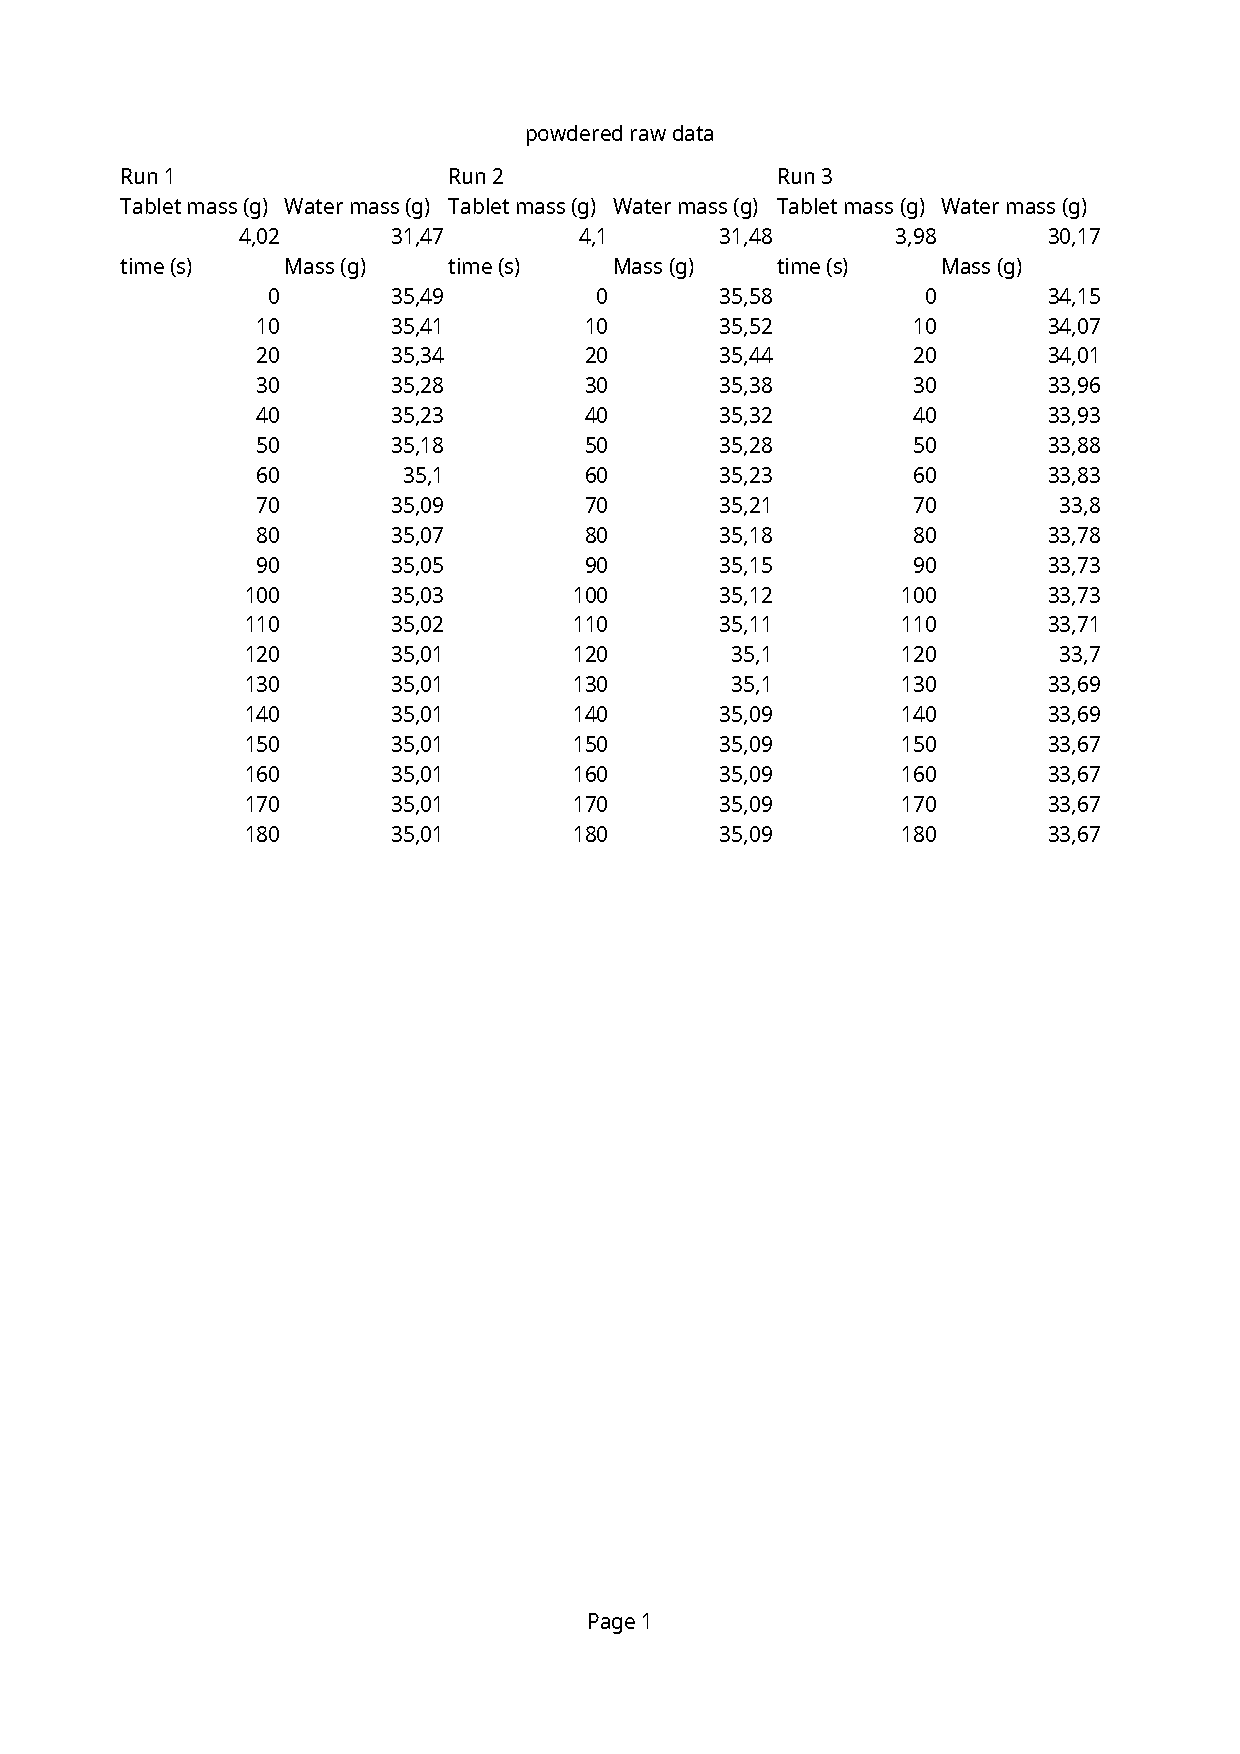
\includepdf[pages=-]{powder.pdf}
	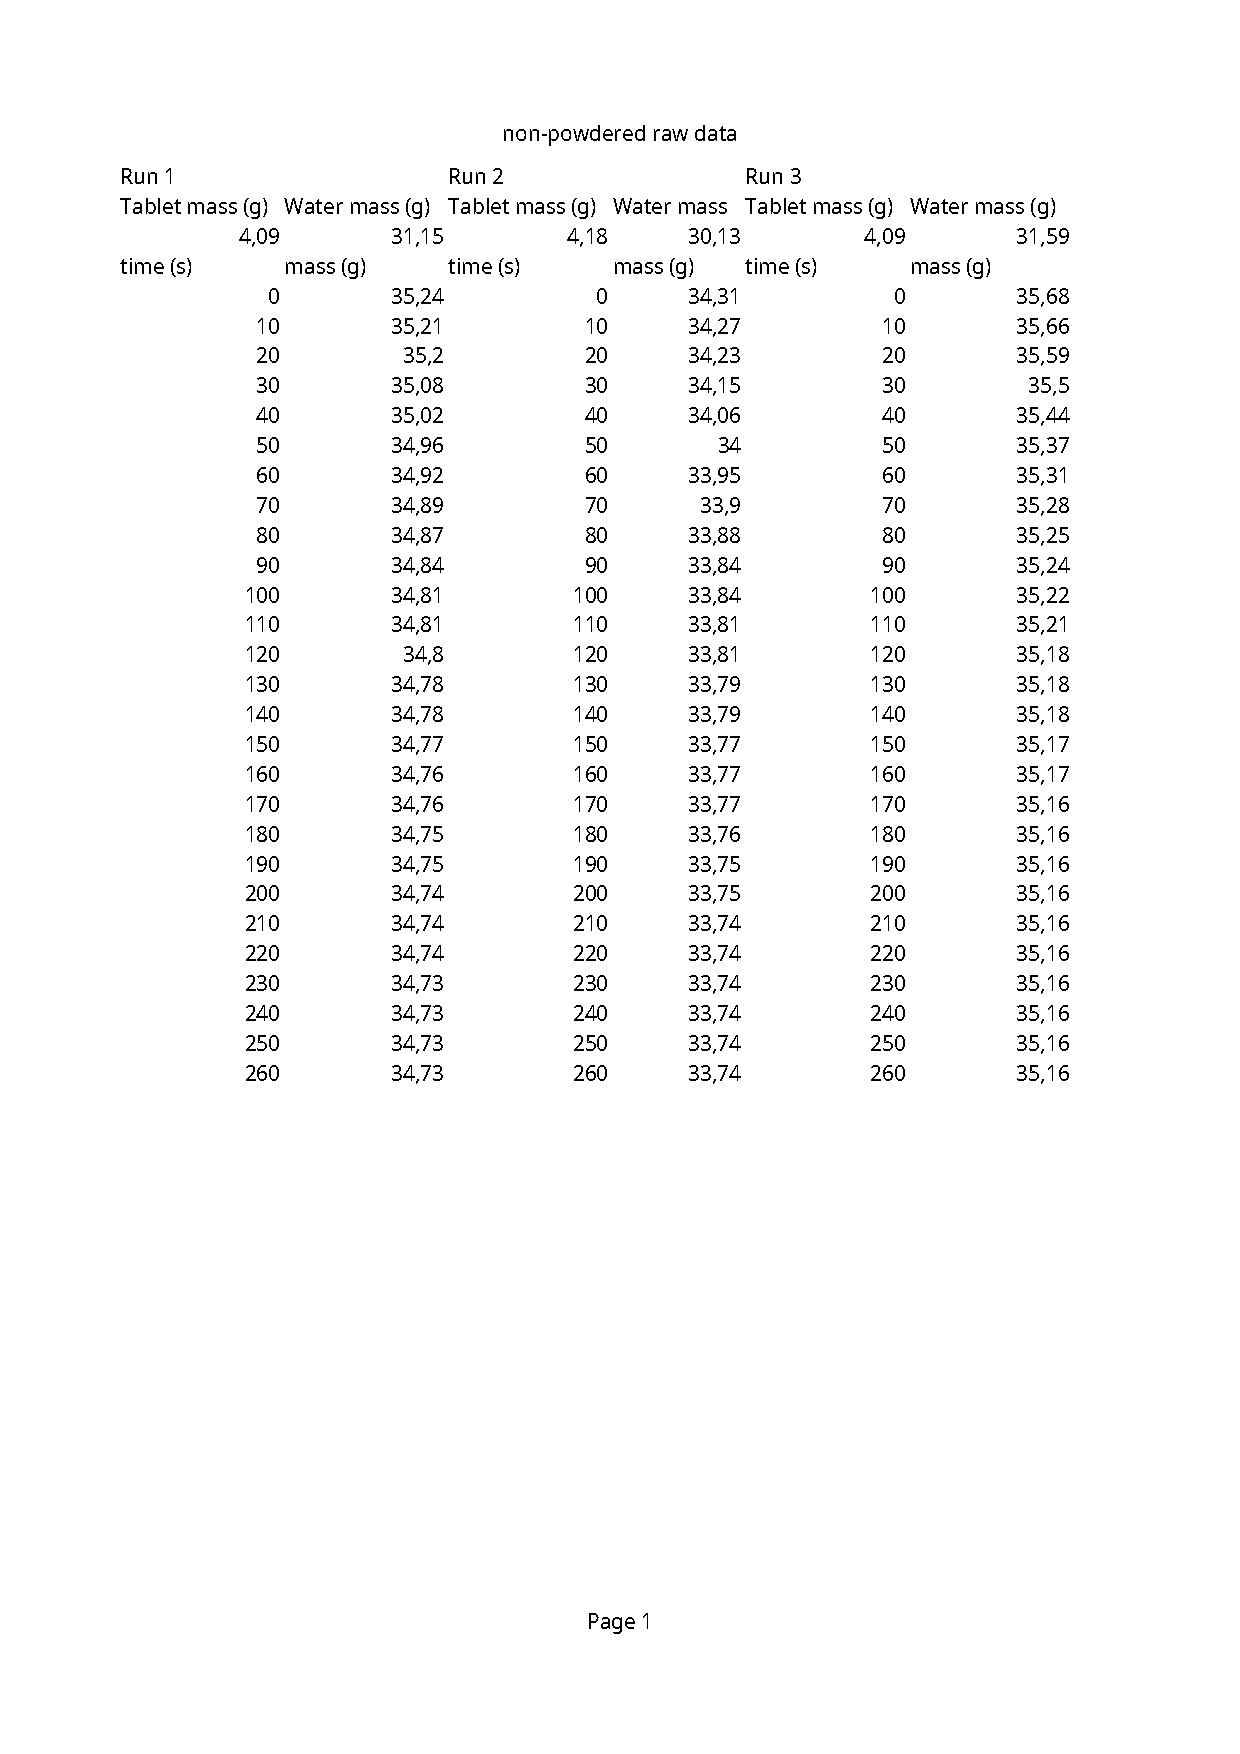
\includepdf[pages=-]{solid.pdf}
\end{document}
